\documentclass[11pt,a4j]{jreport}

\usepackage{comment}
\usepackage{float}
\usepackage{color}
\usepackage{multicol}
\usepackage[dvipdfmx]{pict2e}
\usepackage{wrapfig}
\usepackage{graphicx}
\usepackage{bm}
\usepackage{url}
\usepackage{underscore}
\usepackage{colortbl}
\usepackage{tabularx}
\usepackage{fancyhdr}
\usepackage{ulem}
\usepackage{cite}
\usepackage{amsmath,amssymb,amsfonts}
\usepackage{algorithmic}
\usepackage{textcomp}
\usepackage{xcolor}
\usepackage[ipaex]{pxchfon}
\usepackage[deluxe]{otf}
\usepackage{graphicx}
\usepackage{mathtools}
\usepackage{tikZ}


\usepackage[top=30truemm,bottom=30truemm,left=25truemm,right=25truemm]{geometry}
\renewcommand{\baselinestretch}{1.5}
\usepackage{fancyhdr}
\pagestyle{fancy}

\rhead{チートシート\\あずびわ}
\cfoot{\thepage}
\renewcommand{\headrulewidth}{0.0pt}

\AtBeginDocument{\addtocontents{toc}{\protect\thispagestyle{fancy}}}
\begin{document}
% \textmc{明朝体}

\thispagestyle{empty}
\begin{center}

\vspace{20mm}
{\Large\noindent LaTeX}\\
\vspace{40mm}
{\huge\noindent\textbf{チートシート}}\\
\medskip
\vspace{\baselineskip}
\vspace{30mm}

{\Large\noindent
2024年10月〜\\
\vspace{\baselineskip}
名前:あずびわ\\
}
\vspace{40mm}

\end{center}

\thispagestyle{empty}
\clearpage

%=====================================================================================

% 目次の表示
\tableofcontents
\thispagestyle{fancy}
%=====================================================================================
\pagestyle{fancy}
\lhead{\rightmark}
\renewcommand{\chaptermark}[1]{\markboth{第\ \normalfont\thechapter\ 章~~#1}{}}
\thispagestyle{fancy}
%=====================================================================================
\chapter{LaTeXの基本の使い方}
書きたいこと\\
・表紙周りの設定\\
・パッケージ\\
・beginmathや\$など\\
・エラーが出てきたら 
! LaTeX Error: File `tikZ.sty' not found.\\
\\
・改行\\
・特殊文字はバックスラッシュ入れる\\

\chapter{基本の記法}
\thispagestyle{fancy}
$x^{\prime}+y$\\
$\sigma$\\
$x^{2}$\\
${}~{\forall}x$\\
${}^{\exists}x$
${}_{n}C_{r}$\\
\begin{equation}
a+b
\end{equation}

\chapter{代数学}
\thispagestyle{fancy}
\section{線形代数}
行列の書き方\\
$
\begin{matrix}
    a & b \\
    c & d
\end{matrix}\\
\begin{pmatrix}
    a & b \\
    c & d
\end{pmatrix}\\
$
\subsection{行列式}
$
\begin{vmatrix}
    a & b \\
    c & d
\end{vmatrix}
$

\section{群論}
\subsection{準同型定理}
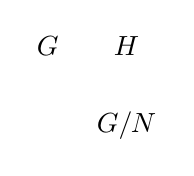
\begin{tikzpicture}
\node(G)   at (0, 1) {$G$};
\node(H)   at (1, 1) {$H$};
\node(G/N) at (1, 0) {$G/N$};
\end{tikzpicture}




\addcontentsline{toc}{chapter}{参考文献}
\renewcommand{\bibname}{参考文献}
\begin{thebibliography}{99}
\end{thebibliography}
山田たろう

\end{document}

